% !TEX program = xelatex

%%% Local Variables: 
%%% coding: utf-8
%%% mode: latex
%%% TeX-engine: xetex
%%% End:

\documentclass[english,handout]{beamer}
\usepackage{pdfpages}
%\pgfpagesuselayout{4 on 1}[a4paper,border shrink=5mm]



\usepackage{mathptmx}
\usepackage[T1]{fontenc}
\usepackage{amsmath}
\usepackage{amssymb}
\usepackage{prftree, bussproofs}
\usepackage{fancyvrb}
\usepackage{soul}
\usepackage{booktabs}


\usepackage{import}
\usepackage{xifthen}
\usepackage{pdfpages}
\usepackage{transparent}

\newcommand{\incfig}[1]{%
    \def\svgwidth{\columnwidth}
    \import{./figures/}{#1.pdf_tex}
}


\usepackage{fontspec}
\setmonofont[Scale=0.9]{FreeMono}

\newtheorem{property}[theorem]{Property}
\newtheorem{axiom}[theorem]{Axiom}

\global\long\def\evidence#1{\left\llbracket#1\right\rrbracket}
\newcommand{\form}[1]{\scalebox{1.087}{\boldmath{#1}}}
\global\long\def\ctx{\text{\ensuremath{\mathcal{\text{Ctx}}}}}%
\global\long\def\set{\text{\textbf{Set}}}%
\global\long\def\ty#1{\text{Ty}\left(#1\right)}%
\global\long\def\tm#1#2{\text{Tm}\left(#1,#2\right)}%

\newcommand{\coe}[2]{\int_{#1}{#2}}
\newcommand{\homo}[3]{\text{Hom}_{#1}\left(#2,#3\right)}
\newcommand{\type}{\mathcal{U}}
\newcommand{\pa}[3]{\texttt{Path}_{#1}\left(#2, #3\right)}
\newcommand{\compt}[5]{\texttt{comp}^{#1} \ {#2} \ \left[{#3} \mapsto{#4} \right] \ {#5}}
\newcommand{\fillt}[5]{\texttt{fill}^{#1} \ {#2} \ \left[{#3} \mapsto{#5} \right] \ {#5}}

\newcommand{\isequiv}[3]{\texttt{isEquiv} \ #1 \ #2 \ #3}

\usepackage{graphicx}

\newcommand{\fig}[2]{
    \begin{figure}\begin{center}\includegraphics[width=0.7\textwidth,height=0.7\textheight,keepaspectratio=true]{figures/#1}\caption{#2\label{#1}}\end{center}
    \end{figure}}

\newcommand{\tcol}[2]{
    \begin{columns}
        \column{.5\textwidth}
        #1
        \column{.5\textwidth}
        #2
    \end{columns}
}

\usepackage{tikz,tikz-cd}
\usepackage{tkz-graph}
\usetikzlibrary{decorations.markings,calc}
\usetikzlibrary{shapes.geometric}

\GraphInit[vstyle = Classic]
\tikzset{
LabelStyle/.style = { %rectangle, %draw,
                        minimum width = 2em, %fill = white!50,
                        text = black, font = \bfseries },
  VertexStyle/.append style = { shape = circle,
  								fill = black,
  								minimum size = 2pt,
  								inner sep=2pt,
                                %font = \Large\bfseries
                                	},
  EdgeStyle/.append style = {->, bend left} }


\pgfdeclarelayer{edgelayer}
\pgfdeclarelayer{nodelayer}
\pgfsetlayers{edgelayer,nodelayer,main}

\tikzstyle{none}=[inner sep=0pt]


\tikzstyle{simple}=[-,draw=black,line width=1.000]
\tikzstyle{arrow}=[-,draw=black,postaction={decorate},decoration={markings,mark=at position 0.5 with {\arrow{>}}}]

\usepackage{graphicx}
\usepackage{multimedia}

\makeatletter
\setbeamercovered{invisible}
%%%%%%%%%%%%%%%%%%%%%%%%%%%%%% LyX specific LaTeX commands.
%% Because html converters don't know tabularnewline
\providecommand{\tabularnewline}{\\}

%%%%%%%%%%%%%%%%%%%%%%%%%%%%%% Textclass specific LaTeX commands.
% this default might be overridden by plain title style
\newcommand\makebeamertitle{\frame{\maketitle}}%
% (ERT) argument for the TOC 
\AtBeginDocument{%
  \let\origtableofcontents=\tableofcontents
  \def\tableofcontents{\@ifnextchar[{\origtableofcontents}{\gobbletableofcontents}]}
  \def\gobbletableofcontents#1{\origtableofcontents}
}

\AtBeginSection[]{
  \begin{frame}
  \vfill
  \centering
  \begin{beamercolorbox}[sep=8pt,center,shadow=true,rounded=true]{title}
    \usebeamerfont{title}\insertsectionhead\par%
  \end{beamercolorbox}
  \vfill
  \end{frame}
}

%%%%%%%%%%%%%%%%%%%%%%%%%%%%%% User specified LaTeX commands.
\usetheme{default}
% or ...dff

%\setbeamercovered{transparent}
% or whatever (possibly just delete it)


\addtobeamertemplate{navigation symbols}{}{%
    \usebeamerfont{footline}%
    \usebeamercolor[fg]{footline}%
    \hspace{1em}%
    \insertframenumber/\inserttotalframenumber{}
}

\makeatother

\usepackage{babel}






% \mode<handout>{%
%     \pgfpagesuselayout{4 on 1}[a4paper] 
%     \setbeameroption{show notes}
% }
% 
% 
% 







\begin{document}
\title[Cubical models for Univalence]{The Constructive Model of \\ Univalence in  Cubical Sets}
\subtitle{Literature review}
\author[W. Vanhulle]{W. Vanhulle\inst{1} \and A. Nuyts\inst{2}\and D. Devriese\inst{3}}
\institute[KUL]{\inst{1}Student \and \inst{2}Supervisor \and \inst{3}Promoter}
\date[30/05/19]{$2^{\text{nd}}$ master thesis presentation (45 min.)}

\makebeamertitle

\pgfdeclareimage[height=0.5cm]{institution-logo}{figures/kuleuven}
\logo{\pgfuseimage{institution-logo}}

\AtBeginSubsection[]{%
  \frame<beamer>{ 
    \frametitle{Outline}   
    \tableofcontents[currentsection,currentsubsection] 
  }
}

%\beamerdefaultoverlayspecification{<+->}
\begin{frame}{Outline}

\tableofcontents{}

\end{frame}

\section{Topology}

\begin{frame}



 \fig{isomorphism}{Hubert-Brierre, 2013}
 
 \begin{itemize}
  \item is the mirror monkey really another monkey?
  \item which properties does he (not) satisfy?
 \end{itemize}

\end{frame}


\begin{frame}
 \fig{isomorphism}{Hubert-Brierre, 2013}
 \begin{quotation}
  They are the same.
 \end{quotation}

\end{frame}



\begin{frame}{Mathematicians are monkeys}

Take two similar objects $A$ and $B$:

\begin{itemize}
 \item Which properties does object $B$ satisfy as well?
 \item Are objects $A$ and $B$ really different?
\end{itemize}


\begin{quotation}
 What is the sameness?
\end{quotation}

\begin{definition}
 An isomorphism is a map that identifies \emph{spaces and their structure}.
\end{definition}


\begin{figure}
\begin{centering}
\begin{table}[]
\begin{tabular}{lll}
\hline
Notation       & Space type         & Isomorphisms                          \\ \hline
$\mathbb{E}^3$ & Euclidean     & rotation, translation, mirroring      \\
$\text{Fin}_n$ & Finite        & permutations                          \\
$G$            & Groups             & homomorphisms                         \\ 
$X$            & Topological & homotopy equivalences
\end{tabular}
\end{table}
\caption{Examples of isomorphisms}
\end{centering}
\end{figure}
 

\end{frame}

\begin{frame}{Isomorphisms in mathematics}

Used for classification of different but similar objects.
%a \emph{weak} identification.

\begin{quotation}
   
    A mathematician is asked by a friend who is a devout Christian: ``Do you believe in one God?'' 
\end{quotation}

    \pause{}
    
    \begin{quotation}
    He answers: ``Yes -- up to isomorphism.'' (© Michael Benjamin Stepp)
\end{quotation}
    
    
%(Equality by definition is \emph{strong})





\end{frame}



\begin{frame}{Homotopy equivalence}


\begin{columns}
    \column{.5\textwidth}
    \fig{mug}{A mug}
    \column{.5\textwidth}
    \fig{donut.jpg}{A donut}
\end{columns}

\begin{definition}[\emph{homotopy equivalent}]
 Can be smoothly deformed into eachother.
\end{definition}
\end{frame}

\begin{frame}{}
 
 \begin{quotation}
 What does a donut think when he sees a mug?
\end{quotation}

\pause

\begin{quotation}
He has the same number of holes.
\end{quotation}



\begin{definition}[homotopy groups]
 Number of \(n\)-dimensional holes 
 
\end{definition}
 
 
 
\end{frame}



\begin{frame}{Computing holes}

homotopy classes of smooth embeddings \[S^n \rightarrow X, \quad \text{or } {[0,1]}^n \rightarrow X\]

\tcol{
                \fig{loops}{A donut has two 1-dimensional homotopy classes.}
}
    {
                \fig{basketball_hollow}{A ball without center has two 2-dimensional homotopy classes.}
}

\end{frame}


\section{Type Theory}

\begin{frame}{Paradox in set theory}{Zermelo, 1899}

The set that contains all sets that do not contain itself:


    \[ R = \{x \mid x \not \in x \}, R\in R \Leftrightarrow R \not \in R \]
    
Weird set
    
    \pause
    
    Paradox eliminated with:
    \begin{itemize}
    \item Universe hierarchy:
        \[\mathcal{U}_0 \in \mathcal{U}_1 \in \ldots \mathcal{U}_{\omega} \in \ldots \]
        
    \item Rejection of ``set comprehension principle'':
    
    \[ S = \{ x \mid P (x ) \} \]
    \end{itemize}
    
    
\end{frame}

\begin{frame}{Constructivism}{Brouwer, 1905}

\begin{quotation}
Mathematics is in essence the result of pure thought.
\end{quotation}

Evolved into constructive logic (Heyting, 1930)

\pause

Type theory (Russel, 1907 -- \ldots):

\begin{itemize}
\item replace sets (and propositions) by types and elements by terms, $$x \in R \Rightarrow x : R$$
\item set universes become type universes
\item constructive logic replaced by formation rules of terms
\end{itemize}

\end{frame}


% \begin{frame}{Present type theory}
%     
%     Two meanings/subfields:
%     \begin{itemize}
%         \item verifying computation in programming languages
%         \begin{figure}
%             \input{figures/haskell.verbatim}
%             \caption{A typed recursive function in Haskell}
%         \end{figure}
%     
%         \pause{}
%         \item alternative constructive foundation of mathematics
%         \begin{figure}
%             \input{figures/agda_comp.verbatim}
%             \caption{Definition of the topological space \(S^1\) in Agda}
%         \end{figure}
%     
%     \end{itemize}
% \end{frame}

\begin{frame}{Type theory as foundation for mathematics}

    Deductive system of judgements with typing rules:


    \begin{prooftree}
        \AxiomC{$\Gamma \vdash f : A \rightarrow B$}
        \AxiomC{$\Gamma \vdash a : A$}
        \BinaryInfC{$\Gamma \vdash b : B$}
    \end{prooftree}

    \begin{itemize}
    \item judgments express that a type is inhabited
    \item all judgements have contexts
    \item typing rules tell how to form and combine types and terms
    \end{itemize}
    
    \begin{definition}[Type-checking]
    Checking if the typing rules are respected.
    \end{definition}
    
\end{frame}


\begin{frame}{Definitional equality}
    
    Definitional equality in type theory (``denoted \texttt{=}'' in code):

    \begin{figure}
    \input{figures/definitional.verbatim}
    \caption{An example of definitional equality.}
    \end{figure}

    \begin{itemize}
     \item used for stating terms, terms and typing rules
     \item defined such that type-checking decidable
    \end{itemize}
    
    
    
\end{frame}

\begin{frame}{Problems definitional equality}

Definitional equality distinguishes  \texttt{0 + m} and \texttt{m + 0}: too \emph{strong} for mathematics.

\begin{quotation}
A weaker alternative?
\end{quotation}

\begin{example}[Leibniz's extensionality axiom]

Functions are identified with values:
     \[f = g \Leftrightarrow f(x) = g(x), \forall x \]
    
    Breaks decidability of type-checking $\Rightarrow$ not possible with definitional equality.
    \end{example}
    

    
    
\end{frame}



\begin{frame}{Identity type}{Martin-L\"of, 1984}

    A type of equality between terms $a,b : X$, denoted $a = b$. Terms $p : (a =b)$ are called ``equalities''.

    \begin{definition}[Introduction rule]
        Given a term $a : X$, there is an equality $\texttt{refl}(a): a = a$.
    \end{definition}

       Elimination rule of equality type:

    \begin{definition}[Induction rule]
            Given the following terms:
        \begin{itemize}
            \item a predicate \(C : \prod_{x,y:A} (x =_A y) \rightarrow \mathcal{U}\)
            \item the base step \(c:\prod_{x:A} C(x,x,\texttt{refl}_x)\)
        \end{itemize}
            there is a function \(f: \prod_{x,y:A} \prod_{p:x=_Ay}C(x,y,p)\) such that \(f(x,x,\texttt{refl}_x) \equiv c(x)\).
        
    \end{definition}

    
\end{frame}

\begin{frame}{Role identity eliminator}

    To prove a property \(C\) that depends on terms $x,y$ and equalities $p:x=y$  it suffices to consider all the cases where
        \begin{itemize}
            \item $x$ is definitionally equal to $y$
            \item the term of the intensional equality type under consideration is $\texttt{refl}_x : x = x$.
        \end{itemize}

        Implications:
        \begin{itemize}
            \item proves transitivity, symmetry
            \item less things equal $\Rightarrow$ weaker than equality ``by definition''.
        \end{itemize}
        
\end{frame}


% \begin{frame}{Short history of HoTT }

% \begin{itemize}
%  \item groupoid model, Hofmann  (1996)
%  \item univalence axiom, Voevodsky (2009)
%  \item univalent foundations, Voevodsky, Grayson, Coquand (2013)
% \end{itemize}

% \begin{figure}[h!]
% \centering    
% 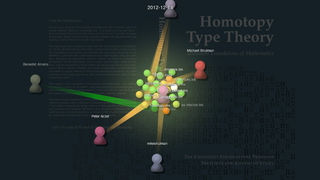
\includegraphics[width=0.7\textwidth]{figures/HoTT-pic.png}
%   \caption{Univalent foundations 2013--2014}
%  \end{figure} 


% \end{frame}

\begin{frame}{Univalence axiom}{Voevodsky, 2009}


\begin{definition}[Type equivalence ]
 Given types $X,Y : \mathcal{U}$ for some universe $\mathcal{U}$, an equivalence $f: X \simeq Y $ of types is a map $f : X \rightarrow Y$ that is a bijection up to equality.
\end{definition}

\begin{quotation}
Equivalences are isomorphisms between topological spaces.
\end{quotation}

\begin{axiom}[Univalence axiom] 
 Given types $X,Y : \mathcal{U}$ for some universe $\mathcal{U}$, the map \(\Phi_{X,Y}: (X=Y) \rightarrow (X \simeq Y)\) is an equivalence of types. 
\end{axiom}

\begin{quotation}
  Equivalences are (up to homotopy equivalence) the same as equalities.
\end{quotation}

Type theory up to isomorphism (homotopy type equivalence)
\end{frame}

\begin{frame}{Consequences of univalence}

\begin{example}[Natural numbers]
$\mathbb{N}$ is a type that behaves like a set.
\begin{itemize}
    \item equivalences \[\mathbb{N} \simeq \mathbb{N}_0 \] are bijections \[\mathbb{N} \leftrightarrow \mathbb{N}_0 \]
    \item univalence implies \[ p : (\mathbb{N} \leftrightarrow \mathbb{N}_0 ) \Rightarrow p : (\mathbb{N} = \mathbb{N})\]

    \item forces multiple equalities $\mathbb{N} = \mathbb{N}_0$
\end{itemize}
\end{example}

\pause

\begin{quotation}
$\Rightarrow$ terms of equality are paths
\end{quotation}

% \begin{figure}[h!]
% \centering    
% 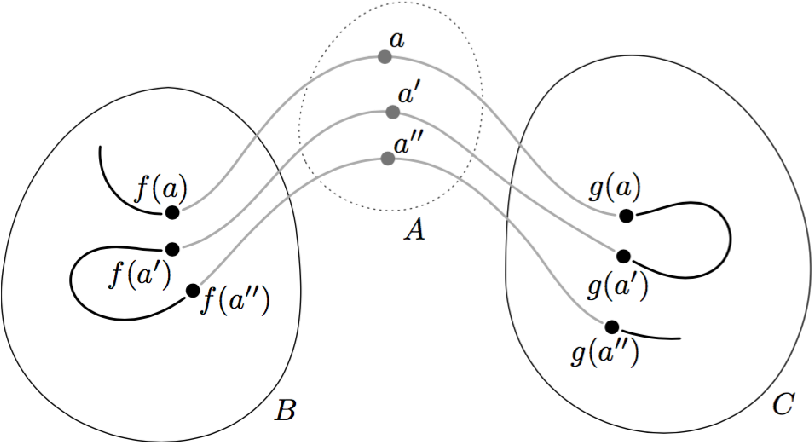
\includegraphics[width=0.5\textwidth]{figures/seifert.png}
%   \caption{Seifert-Van Kampen theorem in HoTT. Hou, Shulman (2016)}
%  \end{figure} 



\end{frame}



\begin{frame}[fragile]
    \frametitle{Consequences of path interpretation}
     
     
     
     
     \tcol{
        A way to construct paths in topology:
        \begin{definition}[Covering]
         A surjective smooth map $\pi : E \rightarrow B$ that is locally homeomorphic.
        \end{definition}

        
        Defining transport:
        \begin{itemize}
            \item take path $p$ in base space $B$ and point $b$ in $\pi^{-1}(p(1))$
            \item path $p$ is lifted to path $p_\star$ ending in $b$
            \item \emph{transport} gives start $p_\star(0)$
        \end{itemize}
        
        More paths means more equalities
        $\Rightarrow$ identity type is indeed \emph{weak}.
        
     }
     {
        \begin{figure}
        \incfig{figures/cover}
        \caption{Based on Jeff Erickson, 2009}
        \end{figure}
        %\fig{cover}{Jeff Erickson, 2009}
     }     
\end{frame}
    

\begin{frame}{Homotopy type theory (HoTT)}{Awodey, 2006}



Gives \emph{homotopy} interpretation to equality type:

%\includegraphics[width=0.8\textwidth]{figures/}
\centering
$$ p,q : a =_X b \quad r,s : p =_{\texttt{Id}_X(a,b)} q$$ 

\begin{tikzpicture}
  [decoration={markings,mark=at position 0.5 with {\arrow{>}}},
   witharrow/.style={postaction={decorate}},
   dot/.style={draw,fill,circle,inner sep=1.5pt,minimum width=0pt}
  ]

  % rectangle 1
  \begin{scope}
     \draw[thick]
       (0,0) coordinate (a1) -- node[left]     {$a$} (0,2) coordinate (d1)
       (2,0) coordinate (b1) -- node[right](q1){$b$} (2,2) coordinate (c1);
     \draw[xstep=2,ystep=1/3] (a1) grid (c1);
     \draw[thick,witharrow] (d1) -- node[above]    {$p$}(c1);
     \draw[thick,witharrow] (a1) -- node[below](f1){$q$}(b1);
  \end{scope}
  
  
  \begin{scope}[shift={(6,0.5)}]
    \node[dot,label={[left] $a$}] (a3) at (0,0) {};
    \node[dot,label={[right]$b$}] (b3) at (4,0) {};
    \draw[thick,witharrow] (a3) to[out=50,in=150]node[above]{$p$} (b3);
    \foreach \o/\i in {40/160,30/170,20/180,10/190,-10/200}
       \draw (a3) to[out=\o,in=\i]  (b3);
    \draw[thick,witharrow] (a3) to[out=-20,in=-130]node[below]{$q$} (b3);
    \draw ($0.5*(a3)+0.5*(b3)$) circle[x radius=2.5,y radius=1.5];
    \node at ($(a3)+(0.5,0.8)$) (X3) {$X$};
    \node at ($(a3)+(0.5,-0.8)$) (X4) {};
  \end{scope}

%connections
  \draw[-stealth,shorten >=4mm] (q1) to[out=30,in=150]node[above]{$r$} (X3);
  \draw[-stealth,shorten >=4mm] (q1) to[out=-30,in=-150]node[below]{$s$} (X4);
\end{tikzpicture} 



$\Rightarrow$ alternative foundation for mathematics based on type theory and topology

\end{frame}




\begin{frame}{Origin univalence}{Grayson, 2018}

\begin{columns}[c]
    \column{.5\textwidth}
        \begin{center}
            \begin{figure}[h!]
                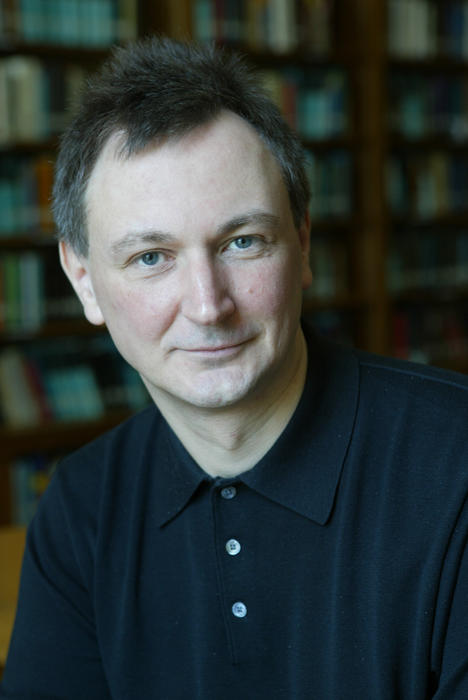
\includegraphics[height=.7\textheight]{figures/voevodsky.jpg}
                \caption{Voevodsky (1966 - 2017)}
            \end{figure} 
        \end{center}
    \column{.5\textwidth}

    \begin{definition}[Univalent type theory]
     Type theory + univalence axiom (also \emph{homotopy type theory})
    \end{definition}


        \pause

        \begin{quotation}
        ... these foundations seem to be faithful to the way in which I think about mathematical objects in my head ...
        \end{quotation}

        faithful = univalent in a Russian translation of Boardman (2006)

\end{columns}
\end{frame}

\begin{frame}{Practical limitations of univalence}
The univalence axiom adds:
\begin{itemize}
    \item intuitive explanation of equality
    \item a definition of equivalence and connection with equality
    \item field of mathematics: HoTT
\end{itemize}

But does not:
\begin{itemize}
    \item make all proofs in mathematics easier or shorter
    \item eliminate need for proofs of equivalence
\end{itemize}




\end{frame}

\begin{frame}{Computing with univalence}{Huber, 2015}

Question posed in 2013:

\begin{quotation}
Can the univalence axiom be implemented in computers such that
\begin{itemize} 
 \item equalities are really paths 
 \item calculations with very simple types as $\mathbb{N}$ still work?
 \end{itemize}
\end{quotation}

Canonicity of $\mathbb{N}$ in cubical type theory:
$$ t \equiv ua ( ... )  \rightsquigarrow u \equiv S ( \dots ( 0 ) \ldots ) : \mathbb{N}  $$



% 
% \begin{quotation}
% Can we, given a term $t: \mathbb{N}$ constructed using the univalence axiom, construct two terms $u : \mathbb{N}$ and $p : t =_{\mathbb{N}} u$ such that $u$ does not involve the univalence axiom?
% \end{quotation}


\end{frame}




\section{Cubical model}

\begin{frame}{Cubical type theory}{Cohen et al., 2015}

A constructive extension of HoTT with dimension variables $i,j,k : \mathbb{I}$ (cubes) as primitives:

\begin{figure}[h!]
    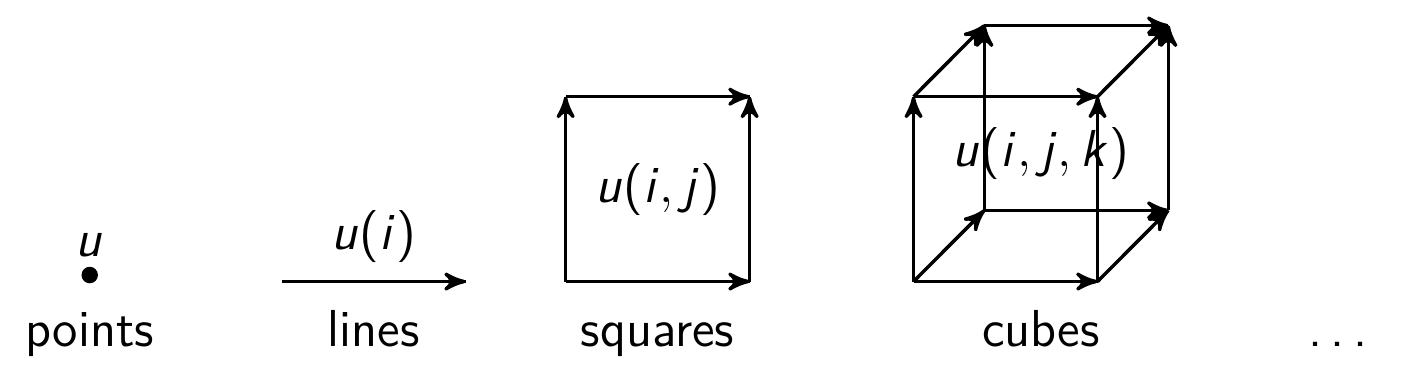
\includegraphics[width=.7\textwidth]{figures/cubes.png}
    \caption{Discrete ``$n$-cubes''. Huber (2016)}
\end{figure}


\begin{itemize}
\item univalence becomes \emph{constructable}
\item computational interpretation for univalence 
\end{itemize}

\end{frame}


\begin{frame}{Are cubes a good idea?}{EnigmaChord, 2016}

\fig{cube-joke.jpg}{}

\pause

\end{frame}


\begin{frame}{Cubes model homotopy}{Altenkirch, Brunerie, Licata, et. al 2013}
 
Homotopy groups are defined as equivalence classes of smooth embeddings:
$$[0,1]^n \rightarrow X$$

\begin{quotation}
In HoTT, higher-dimensional eqalities behave like these embeddings
\end{quotation}
\pause

    \begin{table}[]
        \begin{tabular}{@{}llll@{}}
        \toprule
        Level                & Types                & Cubes                 & Topology               \\ \midrule
        1                    & $p,q : (a = b)$        & edge                  & line                   \\
        2                    & $r,s : (p = q)$        & face                  & path homotopy          \\
        ... & ... & ... & ...   \\
        n                    & ... & n-hypercube           & n-dimensional homotopy \\ \bottomrule
        \end{tabular}
    \end{table}

% \begin{figure}
%  \begin{tikzpicture} [decoration={markings,mark=at position 0.5 with {\arrow{>}}},
   witharrow/.style={postaction={decorate}},
   dot/.style={draw,fill,circle,inner sep=1.5pt,minimum width=0pt}
  ]
		\begin{pgfonlayer}{nodelayer}
		\node [style=none] (0) at (0, -0) {};
		\node [style=none] (1) at (3, -0) {};
		\node [style=none] (2) at (0, 3) {};
		\node [style=none] (3) at (3, 3) {};
		\node [style=none] (4) at (1, 2) {};
		\node [style=none] (5) at (2, 1) {};
		\node [style=none] (6) at (2, 0) {};
		\node [style=none] (7) at (0, 2) {};
		\node [style=none] (8) at (0, 3) {};
		\node [style=none] (9) at (1, 3) {};
		\node [style=none] (10) at (1, 3) {};
		\node [style=none] (11) at (2, 3) {};
		\node [style=none] (12) at (2, 3) {};
		\node [style=none] (13) at (-2, -1) {};
		\node [style=none] (14) at (1, -1) {};
		\node [style=none] (15) at (-4, -0) {};
		\node [style=none] (16) at (-1, -0) {};
		\node [style=none] (17) at (-4, 3) {};
		\node [style=none] (18) at (0.75, -0) {};
		\node [style=none] (19) at (3, 2) {};
		\node [style=none] (20) at (3, 0.75) {};
		\node [style=none] (21) at (0, 1) {};
	\end{pgfonlayer}
	\begin{pgfonlayer}{edgelayer}
		\draw [style=simple] (0.center) to node[left]{$\texttt{P\ 0\ j}$} (2.center);
		\draw [style=arrow] (0.center) to node[above]{$\texttt{P\ i\ 0}$} (1.center);
		\draw [style=simple] (2.center) to node[above]{$\texttt{P\ i\ 1}$} (3.center);
		\draw [style=arrow] (3.center) to node[right]{$\texttt{P\ 1\ j}$} (1.center);
		\draw [style=arrow] (2.center) to node[below]{$\texttt{P}$} (1.center);
		\draw [style=arrow] (13.center) to node[below]{$\texttt{A\ i}$} (14.center);
		\draw [style=arrow] (15.center) to node[left]{\texttt{j}} (17.center);
		\draw [style=arrow] (15.center) to node[below]{\texttt{i}} (16.center);
		\draw [style=arrow] (7.center) to (4.center);
		\draw [style=arrow] (9.center) to (4.center);
		\draw [style=arrow] (11.center) to (5.center);
		\draw [style=arrow] (21.center) to (5.center);
	\end{pgfonlayer}
\end{tikzpicture} 

%  \caption{ \texttt{P} is an equality (homotopy) between equality $A\ i$ and constant equality at $A \ 0$}
% \end{figure}
\end{frame}

\begin{frame}{Operations on cubes}{Bezem, Coquand, Huber et al., 2013}
 
\begin{columns}[c]
    \column{.5\textwidth}
        \begin{center}
            \begin{figure}[h!]
                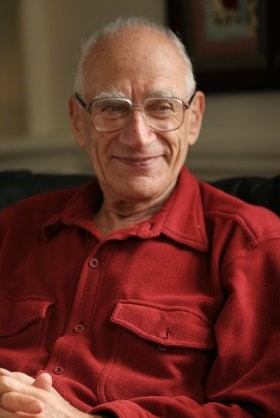
\includegraphics[height=.6\textheight]{figures/kan.jpg}
                \caption{Daniel Kan (1927 --- 2013)}
            \end{figure} 
        \end{center}
    \column{.5\textwidth}
        
        Necessary for modelling HoTT:
        
        \begin{itemize}
         \item  composition $\Rightarrow$ equality type
         \item glueing $\Rightarrow$ univalence
        \end{itemize}


        \begin{figure}[h!]
                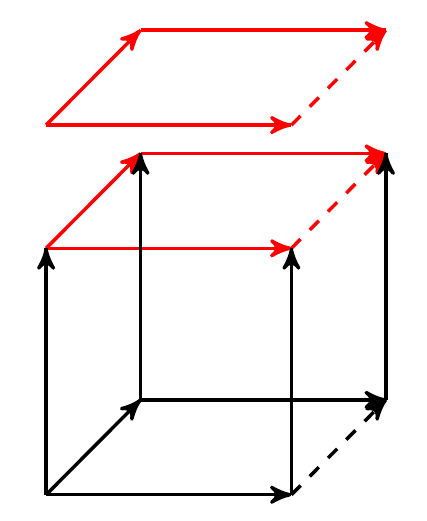
\includegraphics[height=.4\textheight]{figures/extension.png}
        \end{figure} 

        
\end{columns}
\end{frame}




\begin{frame}{Presheaf model on $\mathcal{C}$}{Dybjer, 1994}
 
 
 
 Give interpretation for stuff in type theory:
 \begin{itemize}
 \item base category $\mathcal{C}$ contains ``extra tools'' for model
 \item every context $\Gamma$ is modelled as presheaf on $\mathcal{C}$, denoted $\widehat{\mathcal{C}}$.
 \item types and terms also interpreted in $\widehat{\mathcal{C}}$
\end{itemize}
%  
%  
%  \begin{itemize}
%   \item types are a presheaf \[\widehat{\int_{\mathcal{C}} \Gamma}\]
%   \item terms are elements of $$\prod _{I \in \mathcal{C}, \rho \in \Gamma (I)} A(I,\rho)$$
%  \end{itemize}

 \pause
 Goals:
 
 \begin{itemize}
  \item verify consistency of type theory in sets
  \item justify primitives for implementations
 \end{itemize}
 
Denoted as ``presheaf model $\widehat{\mathcal{C}}$''.

 
\end{frame}

\begin{frame}{Contexts in  presheaf model $\widehat{\mathcal{C}}$}
 
 \begin{definition}[Presheaves $\widehat{\mathcal{C}}$]
     Contravariant functors $\mathcal{C} \rightarrow \mathbf{Set}$
\end{definition}
     
    
    \begin{itemize}
    \item generalize sheaves (see sheafication)
    \item model contexts
    \end{itemize}
    

    \fig{presheaf.png}{A representation of a preseheaf}

\end{frame}
%    
    
   \begin{frame}[fragile]
   \frametitle{Contexts in presheaf model $\widehat{\{0,1\}}$}
\framesubtitle{Hofstra, 2014}
    \begin{example}[Reflexive directed graph]    
    Take $\mathcal{C} = \{0,1\}$ and $\text{Hom}_{\mathcal{C}}= \{B,E,R\}$, $\Gamma \in \widehat{\{0,1\}}$, then 
    
   
%    \tcol{
%       \[ \begin{tikzcd}
% 1
% \arrow[r, bend left, "B"] 
% \arrow[r, bend right, "E"] 
% & 0
% \arrow[l, "R"{above}]
% \end{tikzcd} \]
%     }
%    {
%    \[ \begin{tikzcd}
% \Gamma (1)
% \arrow[r, bend left, "\Gamma (B)"] 
% \arrow[r, bend right, "\Gamma (E)"] 
% & \Gamma(0) 
% \arrow[l, "\Gamma (R)"{above}]
% \end{tikzcd} \]
%     }
    
    Applying functorial identities:
    \begin{figure}
    \begin{centering}
     
\begin{tikzpicture}
  %\SetGraphUnit{5}
  \Vertex[x=0, y=0]{A}
  \Vertex[ x=2,y=0]{B}
  \Edge[](A)(B)
  
  \Vertex[x = 3, y = -1]{C}
  \Vertex[x = 4, y = 1]{D}  
  \Edge[](C)(D)
  \Vertex[x = 5, y = -1]{E}
  \Edge [](C)(E)
  
  \Loop[dist = 1cm, dir = NO](B)
  \Loop[dist = 1cm, dir = NO](A)
  \Loop[dist = 1cm, dir = NO](C)
  \Loop[dist = 0.5cm, dir = NO](D)
  \Loop[dist = 1cm, dir = NO](E)
\end{tikzpicture} 
    
    \end{centering}
    \caption{Reflexive graph}
    \end{figure}
   \end{example} 
\end{frame}

\begin{frame}{Types in  presheaf model $\widehat{\mathcal{C}}$}
    
    
    \begin{lemma}[Types in a presheaf model]
        If $\Gamma \in \widehat{\mathcal{C}}$ a context, then the types are $ \left\{ (\Delta, \sigma) \mid \Delta \in \widehat{\mathcal{C}}, \sigma \in \text{Hom}_{\text{Ctx}}(\Delta , \Gamma) \right\}$.
     \end{lemma}

     
     Helps to characterize types without using presheaves explicitly.
\end{frame}


\begin{frame}{Types in a presheaf model $\widehat{\{0, 1 \}}$}
  \begin{example}[Dependent directed reflexive graph]
  Applying previous lemma to the type $A$ in $\widehat{\{0, 1 \}}$:
\begin{figure}
\centering
  \begin{tikzpicture}
  %\SetGraphUnit{5}
  \Vertex[L = $\rho B$, x=0, y=0]{A}
  \Vertex[L = $\rho E$, x=4,y=0]{B}
  \Edge[label = $\rho$](A)(B)
  \Vertex[L = $(a\rho) B$, x = 0, y = 2]{C}
  \Vertex[L = $(a\rho) E$, x = 4, y = 4]{D}
  
  \Edge[label = $a \rho$](C)(D)
  \Vertex[L = $ (b\rho) E$, x = 4, y =2]{E}
  \Edge [label = $ b \rho$](C)(E)
  \Loop[dist = 1cm, dir = NO, label = $R$, labelstyle=left](C)
  \Loop[dist = 1cm, dir = NO, label = $R$, labelstyle=left](A)
\end{tikzpicture} 

%%\begin{tikzpicture}
%%  %\SetGraphUnit{5}
%%  \Vertex[L = $\rho E$, x=0, y=0]{A}
%%  \Vertex[L = $\rho B$, x=4,y=0]{B}
%%  \Edge[label = $\rho$](A)(B)
%%  \Vertex[L = $(a\rho) E$, x = 0, y = 2]{C}
%%  \Vertex[L = $(a\rho) B$, x = 4, y = 4]{D}
%%  
%%  \Edge[label = $a \rho$](C)(D)
%%  \Vertex[L = $ (b\rho) B$, x = 4, y =2]{E}
%%  \Edge [label = $ b \rho $](C)(E)
%%  \Loop[dist = 3cm, dir = NO, label = $(a\nu)R$](C)
%%  \Loop[dist = 3cm, dir = NO, label = $\nu R$](A)
%%\end{tikzpicture} 
%%

  \caption{The context $\Delta$ above $\Gamma$ representing $A$.}
  \end{figure}
  %\fig{type_lemma}{Modelled by two contexts and a surjective morphism}
 \end{example}


\end{frame}

\begin{frame}{CTT as a presheaf model}
    Dimension variables and cubes have an abstract representation as ``hypercubes'' in a base category:
    
    \fig{cube_presheaf}{Presheaf acting on cubes}

    \begin{itemize}
        \item proves consistency of CTT and HoTT
        \item justifies primitives used in implementations
    \end{itemize}
    
\end{frame}

\begin{frame}{Cube category}

%  In cubical type theory, $\mathcal{C} \not = \{0, 1\}$ but $\mathcal{C} = \square$.
%  
%  \pause 
%  


  \begin{columns}[c]
    \column{.5\textwidth}
        
    \begin{definition}[``Cube'' $\square$]
    Category with:
        \begin{itemize}
            \item objects: $\{ I \mid |I| < \infty , I \subset \mathbb{A} \}$
            \item morphisms $J\rightarrow I$: maps $I \mapsto dM(J)$
            \begin{itemize}
                \item distributive lattice
                \item  $x \wedge 0 = 0, x\vee 1 = 1$
                \item $\neg 0 = 1$ and $ \neg 1 =0$
            \end{itemize}
        \end{itemize}
        \end{definition}
$\mathbb{A}$: countable set of ``dimension variables'' 
    \column{.5\textwidth}
        \fig{lattice}{A simple lattice}
\end{columns}
 
 
\end{frame}

\begin{frame}{Contexts in presheaf model $\widehat{\square}$}
 
    % Base category:
    %     \[\square \equiv \{ I \mid |I| < \infty , I \subset \mathbb{A} \}\]
    % (with special morphisms)

    \begin{example}[Cubical contexts (``cubical sets'')]
        A presheaf $\Gamma \in \widehat{\square}$ is a functor $\square \rightarrow \mathbf{Set}$

        \begin{itemize}
            \item $\Gamma \in \widehat{\square}$ applied to $\{i,j\}$ gives square $\rho \in \Gamma (i,j)$
            \item morphisms in lattice $dM(i,j)$ give corners of $\rho$

        \end{itemize}
        \begin{figure}
            %\incfig{cubical_set}
            
%\documentclass{article}
%\usepackage[utf8]{inputenc}
%\usepackage{tikz}

%\usepackage[active,tightpage]{preview}
%\PreviewEnvironment{tikzpicture}

%\begin{document}


\begin{tikzpicture}[y=0.80pt, x=0.80pt, yscale=-1.000000, xscale=1.000000, inner sep=0pt, outer sep=0pt]
  \path[draw=black,line join=miter,line cap=butt,line width=0.580pt]
    (69.7924,206.3770) -- (69.7924,151.5309) -- cycle;
  \path[draw=black,line join=miter,line cap=butt,line width=0.580pt]
    (69.7924,206.3770) -- (124.6385,206.3770) -- cycle;
  \path[draw=black,line join=miter,line cap=butt,line width=0.580pt]
    (58.8232,162.5001) -- (69.7924,151.5309) -- cycle;
  \path[draw=black,line join=miter,line cap=butt,line width=0.580pt]
    (69.7924,151.5309) -- (80.7617,162.5001) -- cycle;
  \path[draw=black,line join=miter,line cap=butt,line width=0.580pt]
    (124.6385,206.3770) -- (113.6693,195.4077) -- cycle;
  \path[draw=black,line join=miter,line cap=butt,line width=0.580pt]
    (124.6385,206.3770) -- (113.6693,217.3462) -- cycle;
  \path[draw=black,line join=miter,line cap=butt,line width=0.580pt]
    (174.0000,140.5616) .. controls (206.9077,146.0463) and (234.3307,200.8923) ..
    (234.3307,200.8923) .. controls (234.3307,200.8923) and (259.9737,157.0155) ..
    (294.6614,157.0155) .. controls (300.1460,157.0155) and (239.8153,91.2002) ..
    (239.8153,96.6848) .. controls (239.8153,112.1026) and (215.0456,126.5974) ..
    (174.0000,140.5616) -- cycle;
  \path[draw=black,line join=miter,line cap=butt,miter limit=4.00,line
    width=1.741pt] (108.1847,184.4385) .. controls (141.0924,162.5001) and
    (179.4846,162.5001) .. (179.4846,162.5001) -- (179.4846,162.5001) --
    (179.4846,162.5001) -- (179.4846,162.5001) -- (168.5154,151.5309) --
    (179.4846,162.5001) -- (168.5154,173.4693) -- (179.4846,162.5001);
  \path[fill=black,line width=0.580pt] (53.3386,233.8000) node[above right]
    (text1402) {$I = {i, j}$};
  \path[fill=black] (143.6221,188.9764) node[above right] (text1406) {};
  \path[fill=black,line width=0.580pt] (228.8461,151.5309) node[above right]
    (text1410) {$\rho$};
  \path[fill=black,line width=0.580pt] (234.3307,91.2002) node[above right]
    (text1414) {$\rho(i/0)(j/0)$};
  \path[fill=black,line width=0.580pt] (300.1460,162.5001) node[above right]
    (text1418) {$\rho(i/0)(j/1)$};
  \path[fill=black,line width=0.580pt] (228.8461,211.8616) node[above right]
    (text1422) {$\rho(i/1)(j/1)$};
  \path[fill=black,line width=0.580pt] (144.4860,129.5924) node[above right]
    (text1426) {$\rho(i/1)(j/0)$};
  \path[fill=black,line width=0.580pt] (115.1573,163.1877) node[above right]
    (text1430) {$\Gamma$};
  \path[draw=black,line join=miter,line cap=butt,line width=0.580pt]
    (108.9960,89.7490) .. controls (134.6687,80.9556) and (164.9312,75.1435) ..
    (169.3267,52.5291);
  \path[draw=black,line join=miter,line cap=butt,miter limit=4.00,line
    width=1.741pt] (195.9384,102.1694) .. controls (184.9692,85.7156) and
    (168.5154,74.7463) .. (168.5154,74.7463) -- (168.5154,85.7156) --
    (168.5154,74.7463) -- (179.4846,74.7463) -- (168.5154,74.7463);
  \path[fill=black,line width=0.580pt] (190.4538,80.2309) node[above right]
    (text1438) {$(j/0)$};

\end{tikzpicture}
 

            %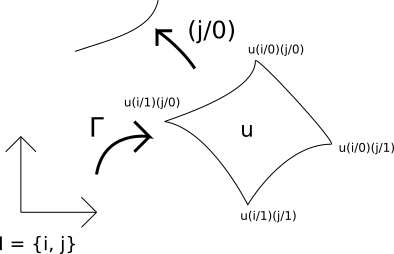
\includegraphics[width=0.6\textwidth]{figures/context}
            
            %\caption{a context }
        \end{figure}
    \end{example}
 
\end{frame}

\begin{frame}{Types in presheaf model $\widehat{\square}$}
    Type $A$ can be represented by a context and a morphism on top of $\Gamma$:
    \begin{itemize}
        \item the $\rho \in \Gamma (i)$ is an edge of a square
        \item endpoints $\rho (0), \rho (1)$ can be lifted to points in the type $u(0),u(1) \in A(i,\rho)$
    \end{itemize}

 \begin{figure}
\centering
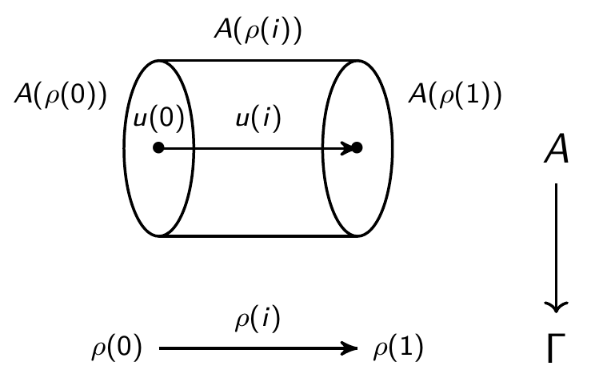
\includegraphics[width=0.7\textwidth]{figures/types}
\caption{A type $A$ within context $\Gamma$. Huber (2016)}
 \end{figure}
 
\end{frame}

\begin{frame}{Partial types in $\widehat{\square}$}{Bezem, Coquand, Huber 2013}
 Partial type $A(i/0)$ is a subtype of $A\ [(i = 0) \mapsto A(i/0)]$ on top of sub-subpolyhedron of cubes $(i=0)\vee (i=1)$:
 
\begin{itemize}
    \item $A$ behaves like a new context $\Delta$ by lemma
    \item partial type $A(i/0)$ is the left side of $A$:
            \fig{types_side}{Huber, 2015}
\end{itemize}

 
 
\end{frame}

\begin{frame}{Other types in presheaf model $\widehat{\square}$}

In the presheaf model on $\square$:
\begin{itemize}
    \item types more complicated
    \item types no longer simply nested graphs
\end{itemize}


Interpreting types in presheaf model $\square$ hard but possible.


\begin{quotation}
 ... transition from interpretation in model to syntax of types
\end{quotation}


\end{frame}

\begin{frame}{Path type}{Bezem, Coquand, 2013}
 
 Syntactical definition of \texttt{Path} type with typing rules:

\begin{prooftree}
\AxiomC{$ i : \mathbb{I} \vdash t : A$}
\AxiomC{$i : \mathbb{I} \vdash t(i/0) = a : A$}
\AxiomC{$i : \mathbb{I} \vdash t(i/1) = b : A$}
\TrinaryInfC{$() \vdash \left< i \right> t : \texttt{Path} \ a\   b$}

\end{prooftree}

% \begin{prooftree}
% \AxiomC{$\Gamma \vdash t : \pa{A}{u_0}{u_1}$}
% \UnaryInfC{$\Gamma \vdash t 0 = u_0 : A$}
% \end{prooftree}
% 
% \begin{prooftree}
% \AxiomC{$\Gamma \vdash t : \pa{A}{u_0}{u_1}$}
% \UnaryInfC{$\Gamma \vdash t 1 = u_1 : A$}
% \end{prooftree}

\begin{itemize}
 \item almost models equality type
 \item not necessarily transitive $\Rightarrow$ composition operation
\end{itemize}


\begin{figure}
\centering
\[ \begin{tikzcd}
a \arrow[r, dashrightarrow] 
& c  \\
a 	\arrow[u, "refl"]	
	\arrow[r, "p \  i"]
& b  \arrow[u, "q \ j"] 
\end{tikzcd}
\] 

\caption{Transitivity can be proven with composition operation.}
\end{figure}

\end{frame}

\begin{frame}{CTT as extension for HoTT}{}
 


 \begin{columns}[c]
    \column{.5\textwidth}
         Other HoTT types interpreted in CTT:
 \begin{itemize}
  \item product, sum types
  \item natural numbers
 \end{itemize}
 
        Univalence proven with concepts from (Streicher, Voevodsky, Kapulkin et al. 2006 -- 2012):
        \begin{itemize}
        \item simplicial sets replaced by cubical sets
        \item partial types and glueing construction conserved
       \end{itemize}
    \column{.5\textwidth}
        \begin{figure}
       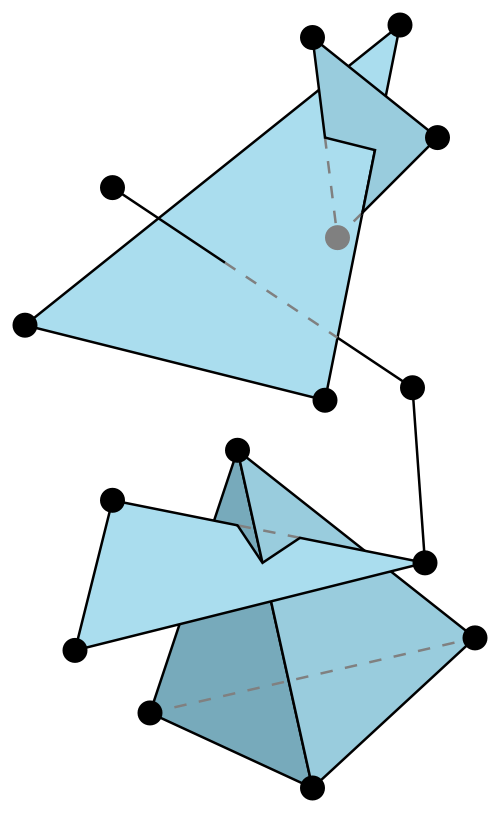
\includegraphics[width=0.7\textwidth]{figures/simplex}
       \caption{Every simplicial complex is a simplicial set}
       \end{figure}
\end{columns}
 
\end{frame}



% \begin{frame}{Equivalences}
%     {Kapulkin, 2012}
  
%   Equivalences $f : T \rightarrow A$ are crucial ingredient for the univalence axiom:
%   \begin{itemize}
%    \item correspond to homotopy equivalences
%    \item have inverse up-to some paths
%   \end{itemize}

  
%    \texttt{Glue} type was introduced to prove univalence:
%    \begin{itemize}
%     \item let \(T\) be a partial type, defined on $i\in \{0,1\}$ 
%     \item glues partial equivalence $f$ and partial type $T$ together:
%    \end{itemize}

%  \fig{glue}{Cohen, 2015}

  
 
% \end{frame}




\begin{frame}{Proving univalence}{Cohen, Coquand, Huber, Moertberg (2015)}

\begin{axiom}[Univalence axiom]
 Given types $X,Y : \mathcal{U}$ for some universe $\mathcal{U}$, there is a map  $\Phi_{X,Y}: (X=Y) \rightarrow (X \simeq Y)$ that is an equivalence of types. 
\end{axiom}


 

\begin{proof}

\begin{enumerate}

\item construction inverse map $\texttt{ua} : (X\simeq Y) \rightarrow (X = Y)$ with \texttt{Glue} construction.

\item for any partial $f : X \rightarrow Y$, $\texttt{Glue} \ [\varphi \mapsto (X, f)] \ Y \simeq Y$

\item for any type $Y$, $\sum_{X} X \simeq Y$ contractible

\item existence of induction principle for $X\simeq Y$.

\item the trivial map $p : X = Y \rightarrow X \simeq Y$ is an inverse ``up-to-path'' of \texttt{ua}
%  
%  $$i : \mathbb{I} \vdash E= \texttt{Glue} \left[ (i=0) \mapsto (X, f),(i=1) \mapsto\left(Y, \texttt{id}_{Y}\right) \right] Y$$
%  
%  $E$ is a path (equality) from $X$ to $Y$.
 
 \end{enumerate}
 
    $\Rightarrow$ the map \texttt{ua}$\equiv \Phi_{X,Y}^{-1}$ is proper inverse and $\Phi_{X,Y}$ equivalence
\end{proof} 

\end{frame}


\begin{frame}[fragile]
\frametitle{Constructing \texttt{ua}}
    \begin{definition}
        $\texttt{ua} : \forall \ X\ Y:\type, X \simeq Y \rightarrow X = Y$
        
        \[ \begin{tikzcd}
        X \arrow[r, dash, dashed, "\texttt{ua}\ f" ] \arrow[d, "f"] & Y  \arrow[d, "\texttt{idEquiv} \ Y"]  \\
        Y\arrow[r, dash, ""] & Y  
        \end{tikzcd}
        \]
        
        
        \end{definition}

    Input: 
    \begin{itemize}
        \item partial equivalence $f$, type $X$
        \item a dimension variable or parameter $i$
    \end{itemize}
    Output: 
    \begin{itemize}
\item $\texttt{ua}\ f \equiv \texttt{Glue} \ [(i = 0) \mapsto (X,f), (i=1) \mapsto (X, \texttt{idEquiv} \ Y)] \ Y$
\item $\texttt{ua}\ f$ is path with endpoints $X$ and $Y$. 
\end{itemize}
\end{frame}

\section{Applications}


\begin{frame}{Applying \texttt{ua} from univalence }
 

 \begin{example}[Monoids]
 
 $$M_1  \equiv (\mathbb{N}, (m,n)\mapsto m+n, 0)$$ and $$M_2 \equiv (\mathbb{N}_0, (m,n)\mapsto m+n -1, 1)$$
\begin{itemize}
 \item  are isomorphic by $$\lambda n \rightarrow n + 1 $$ 
 \item (path-) equal in CTT
\end{itemize}
 
 \end{example}
 

 
\end{frame}

\begin{frame}[fragile]
\frametitle{Encoding the structures in Agda}
%{Building a path}




\begin{figure}
\begin{BVerbatim}
notZero n = Σ ℕ (λ m → (n ≡ (m + 1)))
ℕ₀ = Σ ℕ (λ n → notZero n) 
\end{BVerbatim}
\caption{Definition of $\mathbb{N}_0$ with sum type.}
\end{figure}


\begin{figure}
\begin{BVerbatim}
M₂ : Algebra.Magma _ _
M₂ = record { 
  Carrier = ℕ₀ ;
  _≈_ = (_≡_) ;
  _∙_ = op₂ ;
  isMagma = ... ,
  }
 \end{BVerbatim}
 \caption{Problem reduced to magmas.}
\end{figure}


\end{frame}

\begin{frame}[fragile]
\frametitle{Equality of sets $\mathbb{N} = \mathbb{N}_0$}


\begin{figure}
\begin{BVerbatim}
f : ℕ → ℕ₀ 
f n = (suc n , ( n , refl ) )
\end{BVerbatim}
\caption{Bijections are equivalences for (set-like) types}
\end{figure}

 univalence/\texttt{ua} returns equality \texttt{ℕ ≡ ℕ₀}
 
 
 \begin{figure}
 \begin{BVerbatim}
fEquiv : ℕ ≃ ℕ₀ 
fEquiv = (f ,  isoToIsEquiv (iso f g l' r'))

fEq : ℕ ≡ ℕ₀ 
fEq = ua fEquiv
 \end{BVerbatim}
 \caption{The equality}
\end{figure}

\end{frame}

\begin{frame}[fragile]
\frametitle{Equality of structures $M_1=M_2$}

If $M : M_1 = M_2$, then $\forall i \in [0, 1]$, $M (i)$ magma $\Rightarrow$ point-wise definition:

\begin{itemize}
 \item carrier set $M(i)$ given by $\texttt{fEq i}$
 \item operator $op_i: (m,n) \mapsto m +_i n$ on $M(i)$ is defined with transport of arguments $m,n$ from $\texttt{fEq i}$ to $\mathbb{N}$
\end{itemize}


proofs of magma properties can be transported over $M$: commutativity, etc.




\begin{quotation}
HoTT/univalence/\texttt{ua} gives topological interpretation to invariance of algebraic properties ...
\end{quotation}


\end{frame}

\begin{frame}{Topological transport of arguments}



\begin{figure}
\begin{center}
 \incfig{transport_arguments}
 \caption{Transport of the arguments}
 \end{center}
\end{figure}



\end{frame}
% \begin{frame}{Higher homotopies of spheres}{}
% 
%     Types in HoTT and CTT are topological spaces.
%     Higher homotopy groups compute number of higher-dimensional holes in $S^n$:
% 
%     \fig{groups}{HoTT Book, 2013}
%     Homotopy groups can be defined in CTT as datatypes
% 
% \end{frame}
% 
% 
% \begin{frame}{Implementation in CTT}{Brunerie, 2016}
% 
%  \begin{columns}%[c]
%     \column{.6\textwidth}
%         proven in HoTT with the  univalence axiom:
%         \begin{theorem}
%             $\pi _ 4 (S^3) \cong \mathbb{Z}_n$ for $n=2$ 
% 
%             \end{theorem}
%             \begin{itemize}
%             \item the value $n$ in theorem is implemented in a CTT numeral
%             \item canonicity of numerals predicts normalization 
%             \item normalization fails however
%             \end{itemize}
%         
%         Ongoing optimizations ...
%         
%         \column{.4\textwidth}
%             \begin{figure}
%                 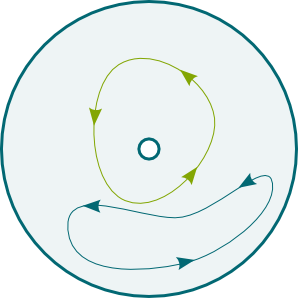
\includegraphics[height=0.4\textheight]{figures/loops}
%                 \caption{The case $S^1$ is simply $\mathbb{Z}$  (drawing from science4all)}
%             \end{figure}
%     \end{columns}
% 
% \end{frame}

\section*{Summary}


\begin{frame}{Conclusion}{Licata, Harper, Cavallo, Orton et al.}
    
    
    \begin{itemize}
        \item HoTT redefines equality
        \item CTT implements HoTT 
        \item HoTT gives formulism for equivalent structures.
    \end{itemize}
    
    Other introductions to cubical type theory: \cite{Huber2016} and \cite{Orton2019}
    
    Recent interesting publications:
    \begin{itemize}
        \item computational type theory is an alternative implementation \cite{Angiuli2018}
        \item composition operation CTT may not be too strong \cite{Cavallo2019}
        \item modelling $\widehat{\square}$ and \texttt{Glue} with language of topoi or other axioms to simplify CTT and composition operations \cite{Orton2017}, \cite{Orton2019} 
    \end{itemize}
    
    
    \end{frame}





\appendix

\section*{Appendix}

\subsection*{For Further Reading}
\begin{frame}[allowframebreaks]{For Further Reading}

  Thanks for watching!

  
  This presentation and full text:
  \url{https://github.com/wvhulle/ctt-presentation}

  
  Source code application:
  \url{https://github.com/wvhulle/transport-magmas}

  
\bibliographystyle{amsalpha}
\bibliography{../../../../Referenties/library}
\end{frame}

\end{document}
